\documentclass[doc,12pt]{apa6}
\usepackage[colorlinks=false]{hyperref}
\usepackage{amsmath}
\usepackage{amssymb}
\usepackage{environ}
\usepackage{enumitem}
\usepackage{threeparttable}
\usepackage{tikz-qtree}
\usepackage{times}
\usepackage{gb4e}

% \linespread{1.5}

\makeatletter
\newsavebox{\measure@tikzpicture}
\NewEnviron{scaletikzpicturetowidth}[1]{%
  \def\tikz@width{#1}%
  \def\tikzscale{1}\begin{lrbox}{\measure@tikzpicture}%
  \BODY
  \end{lrbox}%
  \pgfmathparse{#1/\wd\measure@tikzpicture}%
  \edef\tikzscale{\pgfmathresult}%
  \BODY
}
\makeatother

\title{Homework 3}
\shorttitle{Homework 3}
\author{Edward Hern\'{a}ndez}
\date{26 September 2016}
\affiliation{College of William \& Mary}

\begin{document}
\maketitle

\begin{enumerate}
	\item {}
\end{enumerate}
\vspace*{-36pt}
\begin{center}
\begin{scaletikzpicturetowidth}{\textwidth}
\begin{tikzpicture}[scale=\tikzscale]
	\Tree [.TP [.NP [.Det The ] [.AdjP [.Adj latest ] ] [.N research ] [.PP [.P on ] [.NP [.N dieting ] ] ] ] [.VP [.AdvP [.Adv always ] ] [.V warns ] [.NP [.N people ] ] [.PP [.P about ] [.NP [.Det the ] [.N dangers ] [.PP [.P of ] [.NP [.AdjP [.Adj high ] ] [.N cholestorol ] ] ] ] ] ] ]
\end{tikzpicture}
\end{scaletikzpicturetowidth}
\end{center}

\begin{enumerate}[resume]
	\item
	\begin{enumerate}
		\item V\textsubscript{1}, VP\textsubscript{2}, V\textsubscript{2}, NP\textsubscript{2}, Det\textsubscript{2}, N\textsubscript{2}, PP, P, NP\textsubscript{3}; V\textsubscript{2}, VP\textsubscript{2}
		\item NP\textsubscript{1}, VP\textsubscript{1}
		\item Det\textsubscript{2}, N\textsubscript{2}; Det\textsubscript{2}, N\textsubscript{2}
		\item V\textsubscript{1}, V\textsubscript{2}, Det\textsubscript{2}, N\textsubscript{2}, P, NP\textsubscript{3}
		\item VP\textsubscript{1}
		\item NP\textsubscript{2}, PP
		\item NP\textsubscript{1}
	\end{enumerate}

	\item
	\begin{enumerate}
		\item Inuit appears to be an Ergative-Absolutive language. In the data,
			\textit{tuktu} appears identically as the subject of an
			intransitive verb (b) and as the object of a transitive verb (a).
		\item Russian appears to be a Nominative-Accusative language. In the
			data, the subjects of transitive and intransitive verbs appear to
			be inflected identically (\textit{kniga}, \textit{ja},
			\textit{Ivan}), while the objects of transitive verbs are inflected
			differently (\textit{knigu}, \textit{mnja}, \textit{Ivan'e}).
		\item Nepali appears to exhibit both Accusative and Ergative behavior.
			In the data, the subjects of intransitive verbs lack inflectional
			morphemes (\textit{manis}, \textit{aymay}). In (a) and (b), they
			similarly lack inflectional morphemes as objects, but gain the
			morpheme \textit{-le} as subjects of transitive verbs. This would
			appear to be Ergative-Absolutive behavior. However, in (e) and (f),
			we see transitive verbs take the same nouns, uninflected, as
			subjects. I propose that Nepali is split between Ergative and
			Accusative behavior, and that (e) and (f) exhibit different
			behavior because they are in some way different that (a) and (b),
			perhaps in that their object arguments appear in PPs, or that their
			objects are inanimate.
	\end{enumerate}

	\item
	\begin{enumerate}
		\item \underline{Them} are sleeping.
		\item Do \underline{they} like music?
		\item Sandy doesn't know \underline{them} very well.
		\item Why are \underline{them} talking so loud?
		\item Put \underline{them} on the table, please.
	\end{enumerate}

	\item 
	\begin{enumerate}
		\item
			Often, Juliet says that Romeo lies to his parents. \\
			Juliet says that often Romeo lies to his parents.

		\item \-\\
		\vspace*{-36pt}
		\begin{tikzpicture}
			\Tree [.TP [.NP [.N Juliet ] ] [.VP [.V says ] [.CP [.C that ] [.TP [.NP [.N Romeo ] ] [.VP [.V lies [.PP [.P to ] [.NP [.Det his ] [.N parents ] ] ] ] ] ] ] ] [.AdvP a lot ] ]
		\end{tikzpicture}

		\-\vspace{24pt}

		\begin{tikzpicture}
			\Tree [.TP [.NP [.N Juliet ] ] [.VP [.V says ] [.CP [.C that ] [.TP [.NP [.N Romeo ] ] [.VP [.V lies ] [.PP [.P to ] [.NP [.Det his ] [.N parents ] ] ] [.AdvP a lot ] ] ] ] ] ]
		\end{tikzpicture}

		\item In (3), the AdvP \textit{a lot} is preposed along with the VP.
			This seperates it from the V \textit{says}, preventing it from
			being parsed as part of its VP. In (4), the AdvP is still after
			(and dominated by the VPs of) two Vs, \textit{says} and
			\textit{does}, allowing for two parses (one for each VP which might
			immediately dominate it).
	\end{enumerate}

	\item
	\begin{enumerate}
		\item $NP~\rightarrow{}~N~(Det)$
		\item $VP~\rightarrow{}~V~(NP)~(CP)$
		\item $TP~\rightarrow{}~NP~~VP$

		\item \-\\
		\vspace*{-36pt}
		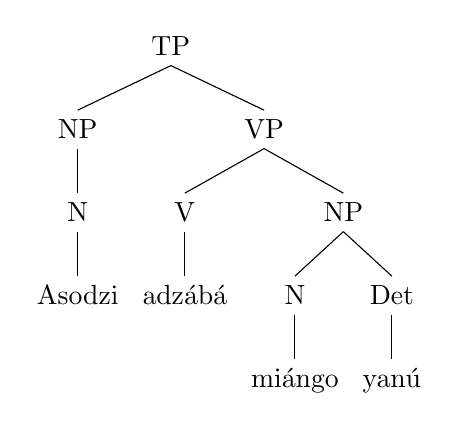
\begin{tikzpicture}
			\Tree [.TP [.NP [.N Asodzi ] ] [.VP [.V adz\'{a}b\'{a} ] [.NP [.N mi\'{a}ngo ] [.Det yan\'{u} ] ] ] ]
		\end{tikzpicture}

		\-\vspace{24pt}

		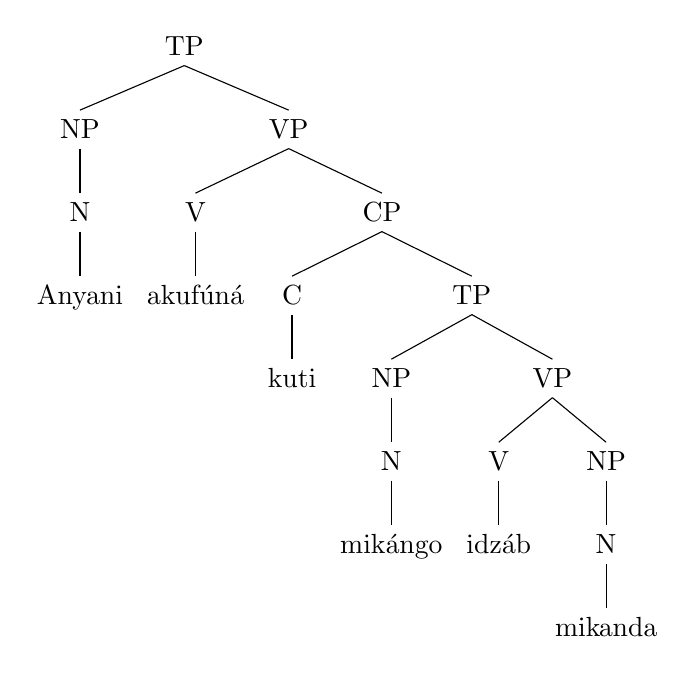
\begin{tikzpicture}
			\Tree [.TP [.NP [.N Anyani ] ] [.VP [.V akuf\'{u}n\'{a} ] [.CP [.C kuti ] [.TP [.NP [.N mik\'{a}ngo ] ] [.VP [.V idz\'{a}b ] [.NP [.N mikanda ] ] ] ] ] ] ]
		\end{tikzpicture}

	\end{enumerate}

\end{enumerate}

% 	\ex \textit{Juliet says that Romeo lies to his parents a lot.}
% 	\begin{xlist}
% 		\ex
% 		\begin{xlist}
% 			\ex fuck
% 			\ex ass
% 		\end{xlist}
% 		\ex no
% 		\ex no
% 	\end{xlist}

% 	\ex
% 	\begin{xlist}
% 		\ex $NP \rightarrow N Det$
% 		\ex $VP \rightarrow V (NP) (CP)$
% 		\ex $TP \rightarrow NP VP$
% 	\end{xlist}

% \end{exe}

\end{document}
